\subsubsection{이진 탐색 트리\translation{binary search tree}} 이진 탐색 트리는 이진 트리의 일종으로서,
각 노드의 왼쪽 서브트리는 해당 노드의 값보다 작은 노드들만, 오른쪽 서브트리는 해당 노드의 값보다 큰 노드들만을 포함하고 있는 트리를 말한다.\cite[pp. 286-287]{CLRS}
이진 탐색 트리에서 원소 삽입과 삭제에 걸리는 시간은 일반적으로 $\mathcal{O}\left(\log n\right)$이다. 또한 트리를 중위 순회($\mathcal{O}\left(n\right)$)할 경우
항상 정렬된 상태로 순회하게 되는 특징이 있다. 따라서 랭킹을 정렬된 상태로 조회해야 하는 쿼리들을 수행하는 데 효율적이므로, 2주차 구현에 이진 탐색 트리르 활용될 수 있다.

\begin{figure}[h]
    \centering
    \subfloat[최악의 경우의 이진 탐색 트리]{
        \resizebox{0.2\linewidth}{!}{%
        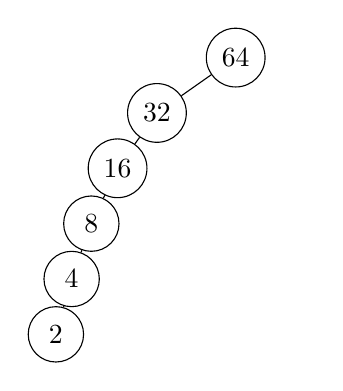
\begin{tikzpicture}[
            every node/.style = {minimum width = 2em, draw, circle},
            level/.style = {sibling distance = 20mm/#1}]
            \tikzset{level distance=20pt}
            \node {64}
            child {node {32} 
                child {node {16} 
                    child {node {8}
                        child {node {4}
                            child {node {2}}
                            child {edge from parent[draw = none]}
                        }
                        child {edge from parent[draw = none]}
                    }
                    child {edge from parent[draw = none]}
                }
                child {edge from parent[draw = none]}
            }
            child {edge from parent[draw = none]};
        \end{tikzpicture}
        }
        \label{fig:bst-worst}
    }%
    \qquad
    \subfloat[최적의 경우의 이진 탐색 트리]{
        \resizebox{0.2\linewidth}{!}{%
        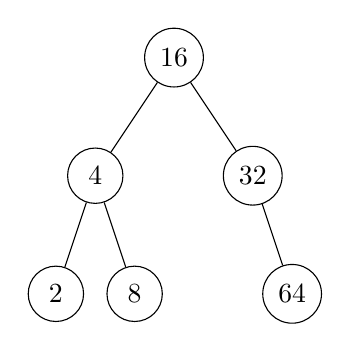
\begin{tikzpicture}[
            every node/.style = {minimum width = 2em, draw, circle},
            level/.style = {sibling distance = 20mm/#1}]
            \node {16}
            child {node {4} 
                child {node {2}}
                child {node {8}}
            }
            child {node {32} 
                child {edge from parent[draw = none]}
                child {node {64}}
            };
        \end{tikzpicture}
        }
    }%
    \caption{최악과 최적의 경우의 이진 탐색 트리}%
    \label{fig:bst}%
\end{figure}

하지만 Figure \ref{fig:bst-worst}의 경우처럼 이진 탐색 트리의 균형이 맞지 않을 경우 최대 $n$개의 노드를 순회해야 하므로
삽입/삭제 연산의 시간 복잡도는 링크드 리스트와 같아지게 된다. 여기에서 자가 균형 이진 탐색 트리\translation{self-balancing binary search tree}를 도입한다면
트리의 높이는 항상 $\left\lceil\log_2 n\right\rceil$가 되고, 최대 $\left\lceil\log_2 n\right\rceil$개의 노드만 순회하게 되므로 평균
$\mathcal{O}\left(\log n\right)$의 시간으로 원소를 삽입 및 삭제할 수 있게 된다.

자가 균형 이진 탐색 트리에는 AVL 트리, red-black 트리 등이 존재한다. C++ STL의 정렬 리스트 자료구조인 \mintinline{c++}{std::set}는 일반적으로
red-black 트리로 구현되어 있으므로\cite{gccset} 여기서도 red-black 트리(이하 RB 트리)를 이용한다.

\begin{figure}[h]
    \begin{center}
        \resizebox{0.65\linewidth}{!}{%
        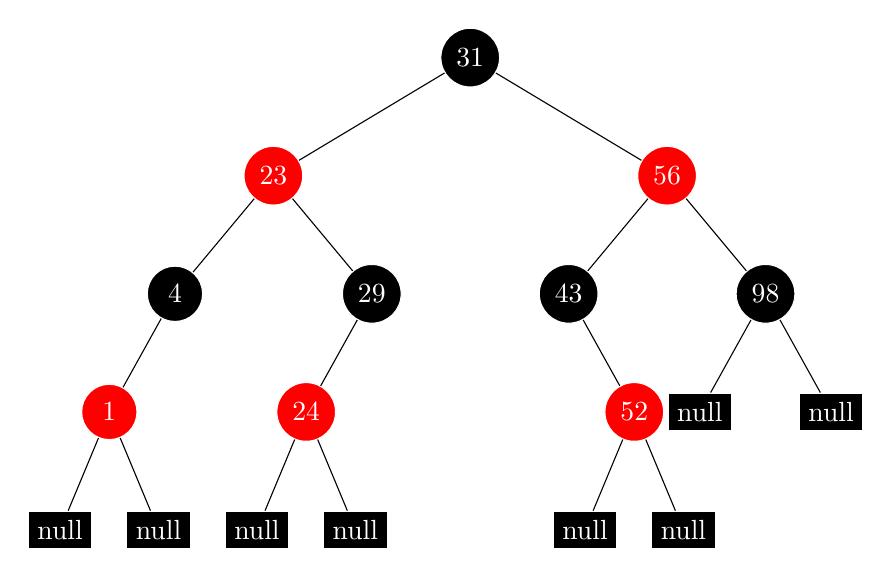
\begin{tikzpicture}[
            every node/.style = {minimum width = 2em, draw, circle, white},
            level/.style = {sibling distance = 50mm/#1}]
            \node[white,fill=black] {31}
            child {node[fill=red] {23} 
                child {node[fill=black] {4}
                    child {node[fill=red] {1}
                        child {node[fill=black,rectangle] {null}}
                        child {node[fill=black,rectangle] {null}}
                    }
                    child {edge from parent[draw = none]}
                }
                child {node[fill=black] {29}
                    child {node[fill=red] {24}
                        child {node[fill=black,rectangle] {null}}
                        child {node[fill=black,rectangle] {null}}
                    }
                    child {edge from parent[draw = none]}
                }
            }
            child {node[fill=red] {56}
                child {node[fill=black] {43}
                    child {edge from parent[draw = none]}
                    child {node[fill=red] {52}
                        child {node[fill=black,rectangle] {null}}
                        child {node[fill=black,rectangle] {null}}
                    }
                }
                child {node[fill=black] {98}
                    child {node[fill=black,rectangle] {null}}
                    child {node[fill=black,rectangle] {null}}
                }
            };
        \end{tikzpicture}
        }
        \caption{Red-black 트리의 예시}
    \end{center}
\end{figure}


RB 트리는 이진 탐색 트리에 더해 다음과 같은 성질들이 추가로 적용되는 트리이다.\cite[pp. 308-309]{CLRS}
\begin{itemize}
    \item 노드는 null일 수 있다.
    \item 각 노드의 색은 빨강, 검정 중 하나이다. 루트 노드나 null 노드는 항상 검정색이다.
    \item 어떤 노드가 빨강색일 경우 자식 노드는 모두 검정색이다.
    \item 임의의 노드에서 리프 노드까지의 모든 경로에는 같은 수의 검정 노드가 있다.
\end{itemize}
루트에서 리프 노드까지의 최단 경로가 모두 검정 노드로만 구성되어 있다고 했을 때, 최장 경로는 검정 노드와 빨강 노드가 번갈아 나오는 경로가 된다.
임의의 노드에서 리프 노드까지의 모든 경로에는 같은 수의 검정 노드가 있다고 했고, 빨강 노드의 자식은 무조건 검정 노드이므로
모든 경로에 대해 최장 경로의 거리는 최단 경로의 거리의 두 배 이상이 될 수 없게 된다.

\subsubsection{결정 트리\translation{decision tree}} 결정 트리는 의사 결정 규칙과 결과를 트리 구조로 도식화한 트리이다. 결정 트리로 미래의 가능한 보드 상태들과 그 때의 결과를 저장하고 관리하면
볼 수 있는 미래의 상태 공간을 쉽게 탐색할 수 있으므로 이를 이용해 3주차의 추천 알고리즘을 구현할 수 있다.

\subsubsection{가지치기\translation{pruning}} 가능한 모든 상태에 대한 완전 결정 트리는 그 구성과 탐색에 많은 시간과 공간을 필요로 하므로, 가능성이 떨어지는 노드들을 삭제하는 방법으로 가지치기를
할 수 있다.

\begin{figure}[h]
    \begin{center}
        \resizebox{0.65\linewidth}{!}{%
        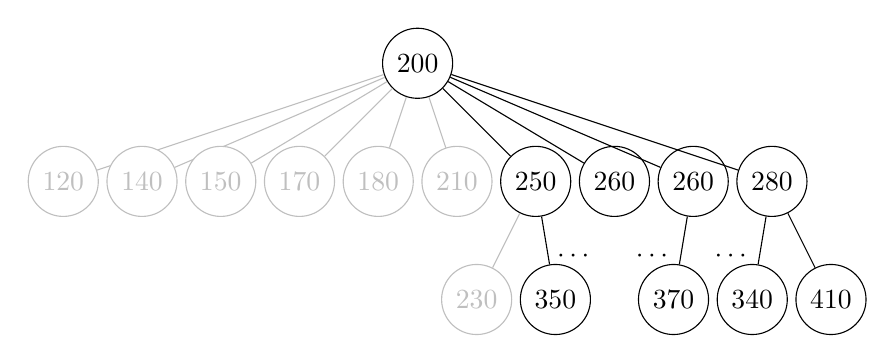
\begin{tikzpicture}[
            every node/.style = {minimum width = 2em, draw, circle, fill=white},
            level/.style = {sibling distance = 10mm/#1}]
            \node {200}
            child {node[text=lightgray, draw=lightgray] {120}[text=lightgray, draw=lightgray]}
            child {node[text=lightgray, draw=lightgray] {140}[text=lightgray, draw=lightgray]}
            child {node[text=lightgray, draw=lightgray] {150}[text=lightgray, draw=lightgray]}
            child {node[text=lightgray, draw=lightgray] {170}[text=lightgray, draw=lightgray]}
            child {node[text=lightgray, draw=lightgray] {180}[text=lightgray, draw=lightgray]}
            child {node[text=lightgray, draw=lightgray] {210}[text=lightgray, draw=lightgray]}
            child {node {250}
                child{node[text=lightgray, draw=lightgray]{230}[text=lightgray, draw=lightgray]}
                child{edge from parent[draw = none]}
                child{node{350}}
                child{edge from parent[draw = none] node[fill=none, draw=none]{$\cdots$}}
            }
            child {node {260}
                child{edge from parent[draw = none]}
                child{edge from parent[draw = none]}
                child{edge from parent[draw = none]}
                child{edge from parent[draw = none] node[fill=none, draw=none]{$\cdots$}}
            }
            child {node {260}
                child{edge from parent[draw = none]}
                child{node{370}}
                child{edge from parent[draw = none]}
                child{edge from parent[draw = none] node[fill=none, draw=none]{$\cdots$}}
            }
            child {node {280}
                child{edge from parent[draw = none]}
                child{node{340}}
                child{edge from parent[draw = none]}
                child{node{410}}
            };
        \end{tikzpicture}
        }
        \caption{결정 트리에서 레벨당 최대 4개의 노드만 남기고 가지치기한 모습}
        \label{fig:pruning}
    \end{center}
\end{figure}

Figure \ref{fig:pruning}의 경우 각 노드마다 10개의 자식 노드가 있는 트리이다. $n$개의 레벨에 대해 이 트리의 공간 복잡도는 $\mathcal{O}\left(10^n\right)$이다.
하지만 각 레벨마다 회색으로 표시된 노드들은 삭제하고 최대 4개의 노드만 남긴다면 공간 복잡도는 $\mathcal{O}\left(n\right)$이 되는 것을 확인할 수 있다.

가지치기의 구체적인 방법은 너비 우선 탐색과 퀵 정렬 항목에 기술한다.

\subsubsection{너비 우선 탐색\translation{breadth-first search}}
너비 우선 탐색이란 그래프에서 임의의 노드에서 탐색을 시작해 가장 멀리 떨어져 있는 정점을 나중에 탐색하는 알고리즘이다.

트리에서 루트 노드를 레벨 0으로 두고, 레벨 $n$인 노드의 자깃 노드의 레벨을 $n+1$으로 둔다면 너비 우선 탐색을 사용할 경우 탐색 순서는 레벨이 작은 정점에서 높은 정점 순으로 진행되게 된다.
추천 알고리즘의 경우 현재 상태를 전부 탐색한 후 다음 블록이 놓이고 난 상태를 전부 탐색하고, 그 후에 그 다음 블록이 놓인 상태를 전부 탐색하는 식으로 동작하게 되는데 결정 트리의 각 레벨마다
노드 개수의 상한선을 유지하면서 동적으로 트리를 생성하려면 너비 우선 탐색법이 효율적이다.

결정 트리의 한 레벨을 탐색하고, 노드들을 효율적인 결과 순으로 정렬해 상한선만큼만 남기고 가지치기한 후,
남은 노드들에 대해서만 다음 레벨을 생성하고 탐색하는 식으로 결정 트리의 시공간 복잡도를 지수 복잡도에서 선형 복잡도로 개선할 수 있다.

\subsubsection{퀵 정렬\translation{quicksort}} 가지치기를 할 때 상위 몇 개의 값을 가지는 노드를 골라내기 위해서는 정렬을 하는 것이 효율적이다.
퀵 정렬은 분할 정복법\translation{divide and conquer method}을 이용한 정렬 알고리즘\cite[p. 181]{CLRS}이다.

퀵 정렬을 하기 위해서는 우선 어떤 리스트에서
임의의 원소를 골라 피벗으로 설정하고, 피벗 앞에는 피벗보다 큰 값을, 뒤에는 피벗보다 작은 값을 놓는다. 그리고 피벗을 기준으로 왼쪽을 하나의 리스트로, 오른쪽을 하나의 리스트로 보고
각각의 리스트에 대해 재귀적으로 퀵 정렬을 수행한다.

버블 정렬이나 삽입 정렬은 $n$개의 원소를 정렬하는 데에 $\mathcal{O}\left(n^2\right)$의 시간이 걸리는 데 반해 퀵 정렬은 
평균적으로 $\mathcal{O}\left(n \log n\right)$의 시간이 걸리는 효율적인 알고리즘이다.\cite[p. 181]{CLRS}

\subsubsection{발견법\translation{heuristic}적 알고리즘} 완전 최적해를 찾는 것은 시공간적 한계에 의해 무리가 있으므로 현재의 여러 상황을 고려해
최적해일 확률이 높은 쪽으로 결정하는 알고리즘을 사용할 수 있다.

\textit{Classic Tetris World Championship}(CTWC)은 여러 플레이어가 NES\translation{Nintendo Entertainment System} 테트리스에서
게임 오버 직전까지 달성한 점수로 겨루는 토너먼트 대회이다. CTWC 결승 플레이어들은 왼쪽 9줄에는 블럭을 최대한 구멍 없이 쌓고, 남겨 둔 오른쪽 1줄에 I 블록을 끼워넣음으로서
4라인 클리어를 최대화시키는 전략을 사용하는 것을 확인할 수 있다.\cite{CTWC}

\begin{wrapfigure}{r}{0.4\textwidth}
    \OMINO{%
    ............+-+..\\%
    ............|Z|..\\%
    ..+---+...+-+.|..\\%
    ..|L.L|...|Z.Z|..\\%
    +-+-+.+---+.+-+-+\\%
    |X.X|L|X.X|Z|X.X|\\%
    |...|.|...+-+...|\\%
    |X.X|L|X.X|.|X.X|\\%
    +---+-+---+.+---+\\%
    }
    \caption{깊이 2의 골짜기}
    \label{fig:valley}
\end{wrapfigure}

    
따라서 점수를 통해 추천 위치를 판단하는 것보다는 보드 상태에 대해 여러 기준을 두고, 이를 바탕으로 추천하는 것이 바람직함을 알 수 있다. 4라인 클리어를 최대화하기
위해서 다음과 같은 휴리스틱을 설정할 수 있다.

\begin{itemize}
    \item 현재 4라인 클리어가 가능한가의 여부
    \item 현재 상태에서 클리어되는 줄 수
\end{itemize}

블록을 안정적으로 배치하려면 현재 필드에 구멍이 적어야 하며 높이가 평탄해야 하고, 비교적 낮은 위치에 블록을
놓는 게 바람직하다.

특히 이웃한 행들의 높이보다 낮은 높이를 갖는 행을 `골짜기'라고 정의한다면,
Figure \ref{fig:valley}에서 보이듯이 높이 2 이상의 골짜기에는 L, J 블록만, 높이 3 이상의 골짜기에는
I 블록만 놓아야 필드 중간에 구멍이 생기지 않는다.
필드 중간에 구멍이 생기면 비효율적이므로 너무 높은 골짜기가 생기는 것은 가급적 피해야 좋을 것이다.

따라서 블록의 안정적 배치를 위해 다음과 같은 휴리스틱들을 추가로 설정할 수 있다.

\begin{multicols}{2}
    \begin{itemize}
        \item 현재 블록이 놓인 $y$ 좌표
        \item 모든 행의 높이의 합
        \item 모든 행의 이웃한 행과의 높이의 차이의 합
        \item 가장 높은 행과 가장 낮은 행의 높이의 차이
        \item 가장 낮은 행의 높이
        \item 구멍의 수
        \item 구멍에서 바닥까지의 거리의 합
        \item 구멍에서 표면까지의 거리의 합
        \item 가장 낮은 구멍의 $y$ 좌표
        \item 가장 높은 구멍의 $y$ 좌표
        \item 골짜기의 높이의 합
        \item 높이 3 이상의 골짜기의 수
        \item 모든 열에 대해 이웃하게 연결되어 있는 셀 요소들의 개수
    \end{itemize}
\end{multicols}

높이가 낮을 때는 4라인 클리어를 하기 위해 스택을 쌓는 것이 효율적이지만, 높이가 높은데 I 블록이 안 나온다면 게임오버를 당할 확률이 높아진다.
이를 막기 위해 다음과 같은 휴리스틱을 추가로 설정한다.

\begin{itemize}
    \item 현재 필드의 총 셀의 개수
    \item 현재 필드의 모든 셀의 높이의 합
    \item $y$ 좌표가 10 이하인 모든 셀의 높이의 합
\end{itemize}

\subsubsection{담금질 기법\translation{simulated annealing}} 담금질 기법은 전역 최적화 문제에 대한 확률적 메타 알고리즘이다. `담금질 기법'이라는 이름의 유래는
금속 공학의 풀림\translation{annealing}의 오역에서 비롯되었는데, 풀림은 금속 재료를 가열한 다음 조금씩 냉각해 결정을 성장시켜 그 결함을 줄이는 작업이다.
열에 의해서 원자는 초기의 위치로부터 멀어져 에너지가 더욱 높은 상태로 추이되며, 금속을 천천히 냉각함으로써 원자는 초기 상태보다 내부 에너지가 한 층 더 극소인 상태를
얻을 가능성이 많아진다. 담금질 기법은 이런 현상과 비슷한 원리로 큰 탐색 공간에서 어떤 함수의 전역 최적해\translation{global optima}에 대한 근사를 진행하는 과정이다.\cite{1981Khachaturyan}

예를 들어 어떤 벡터 $\mathbf{v} = \left<a,\,b\right>$에 대해 보드의 점수가
$f\left(\mathbf{v}\right) = a\times\mbox{(줄 클리어 수)} - b\times\mbox{(묻힌 구멍 수)}$로 계산된다면, 기준으로 삼았을 때 가장 좋은 결과를 주는 $\mathbf{v}$를 찾는 것은 쉬운 일이 아니다.
여러 휴리스틱을 사용해 벡터의 차원이 늘어난다면 더 그러하다. 실제로 이 프로젝트의 추천 시스템은 18개의 휴리스틱을 사용하고 있어, 18차원 계수 벡터 형태의 최적해 산출이 필요하다.
이 기법은 해를 반복해 개선함으로써, 현재의 해 근방에 있는 해를 임의로 찾아가는 방법으로 최적인 $\mathbf{v}$의 근사값을 구할 수 있다.

`에너지'를 일종의 비용 함수\translation{cost function}으로 정의하자. 임의의 온도 $T$를 설정하고, 현재 상태의 에너지 $e_1$, 현재 상태 주변의 계수들을 이용해 계산한
랜덤 상태의 에너지 $e_2$를 비교하여 확률 $p=\exp \left(\dfrac{e_1-e_2}{kT}\right)$를 얻는다.
이 때 $k$는 상수이다. 여기서 0과 1 사이에서 얻은 무작위의 실수 $r$에 대해, $p>r$이면 현재 상태를 새 상태로 바꾼다. 마지막으로 $k$에 온도 감률을 곱한다. 이 과정을 $T$가 임계 온도 이상일 경우 계속 반복한다.

만약 $e_1 \geq e_2$라면 새로운 상태가 기존 싱태보다 에너지가 낮음을 의미하므로 새로운 상태의 계수를 사용하는 것이 이득이다. 한편 $e_1 > e_2$일 경우 에너지가 더 높아지는데,
이 상태는 탐욕법\translation{greedy algorithm}을 쓸 경우 무조건 무시되는 상태이지만, 에너지가 높은 상태를 거쳐야만 다시 작은 상태가 나오는 경우도 무시할 수 없으므로
위에서 계산한 $p$의 확률로 에너지가 높은 경우에도 탐색을 진행한다.